\chapter*{Proposition 38}



\begin{figure*}[ht]
    \begin{center}
    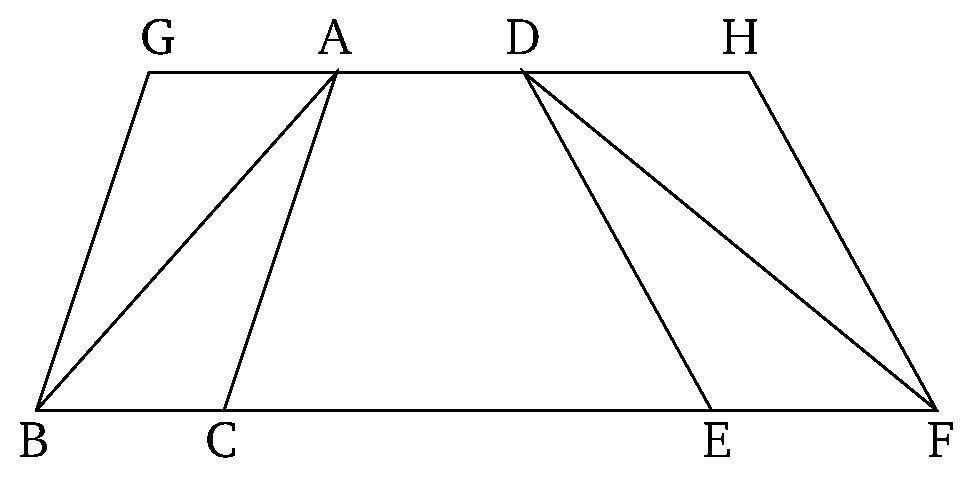
\includegraphics[width=0.5\linewidth]{figures/fig38e.eps}
    \label{fig:prop_38}
    \end{center}
\end{figure*}

Triangles which are on equal bases and between the same parallels
are equal to one another.

Let $ABC$ and $DEF$ be triangles on the equal bases $BC$ and $EF$, and between the same parallels $BF$ and $AD$. I say that triangle $ABC$ is equal to triangle $DEF$.

For let $AD$ have been produced in both directions to $G$ and $H$, and
let the (straight-line) $BG$ have been drawn through $B$ parallel to $CA$ [Prop.~1.31], and let the (straight-line) $FH$ have been drawn through
$F$ parallel to $DE$ [Prop.~1.31]. Thus,  $GBCA$ and $DEFH$ are
each parallelograms. And $GBCA$ is equal to $DEFH$.
For they are on the equal bases $BC$ and $EF$, and between  the same
parallels $BF$ and $GH$ [Prop.~1.36]. And triangle $ABC$ is half of the parallelogram
$GBCA$. For the diagonal $AB$ cuts the latter in half [Prop.~1.34]. And
triangle $FED$ (is) half of parallelogram $DEFH$. For the diagonal $DF$ cuts
the latter in half. [And the halves of equal things are equal to one another.] Thus,
triangle $ABC$ is equal to triangle $DEF$.

Thus, triangles which are on equal bases and between the same parallels
are equal to one another. (Which is) the very thing it was required to show.



\section*{Commentary}

\begin{proposition}\label{proposition_38}\lean{Elements.Book1.proposition_38}\leanok
    If
\end{proposition}
\begin{proof}
    \uses{proposition_31,proposition_34,proposition_36}\leanok
\end{proof}
